\documentclass[tikz,border=5pt]{standalone}

\begin{document}

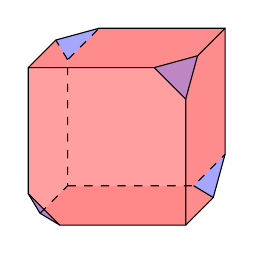
\begin{tikzpicture}

\fill[draw=none, red!50, opacity=0.9] (-0.5, -0.5) -- (1.1,-0.5) -- (1.5, -0.1) -- (1.5,1.5) -- (-0.1,1.5) -- (-0.5, 1.1) -- cycle; 
\fill[draw=none, red!50, opacity=0.9] (-0.85, -0.85) -- (-0.5,-0.5) -- (-0.5,1.1) -- (-0.65, 1.35) -- (-1,1) -- (-1,-0.6) -- cycle;
\fill[draw=none, red!30, opacity=0.5] (-1,-0.6) -- (-0.6,-1) -- (1,-1) -- (1,0.6) -- (0.6,1) -- (-1,1) -- cycle;
\fill[draw=none, red!50, opacity=0.9] (-0.6, -1) -- (1,-1) -- (1.35, -0.65) -- (1.1, -0.5) -- (-0.5, -0.5) -- (-0.85, -0.85) -- cycle;
\fill[draw=none, blue!50, opacity=0.7] (1.35, -0.65) -- (1.1, -0.5) -- (1.5, -0.1) -- cycle;
\fill[draw=none, blue!50, opacity=0.7] (-0.5, 1.1) -- (-0.65, 1.35) -- (-0.1,1.5) -- cycle;
\fill[draw=none, blue!50, opacity=0.6] (-1,-0.6) -- (-0.6, -1) -- (-0.85,-0.85) -- cycle;
\fill[draw=none, blue!50, opacity=0.5] (1, 0.6) -- (0.6, 1) -- (1.15, 1.15) -- cycle;
\draw[-] (-1,-0.6) -- (-0.6,-1) -- (1,-1) -- (1,0.6) -- (0.6,1) -- (-1,1) -- cycle;
\draw[-] (-1, -0.6) -- (-0.85,-0.85) -- (-0.6, -1);
\draw[dashed] (-0.85,-0.85) -- (-0.5,-0.5) -- (-0.5,1.1) -- (-0.1, 1.5);
\draw[dashed] (-0.5, 1.1) -- (-0.65, 1.35);
\draw[-] (-1,1) -- (-0.65, 1.35) -- (-0.1,1.5) -- (1.5,1.5) -- (1.5, -0.1);
\draw[-] (0.6,1) -- (1.15, 1.15) -- (1.5,1.5);
\draw[-] (1,0.6) -- (1.15, 1.15);
\draw[dashed] (-0.5, -0.5) -- (1.1, -0.5) -- (1.5, -0.1);
\draw[-] (1,-1) -- (1.35, -0.65) -- (1.1, -0.5);
\draw[-] (1.35, -0.65) -- (1.5, -0.1);
\end{tikzpicture}
\end{document}